\documentclass[]{article}

\usepackage[utf8]{inputenc}

\usepackage[T1]{fontenc}

\usepackage[english]{babel}

\usepackage{amsmath, amsfonts, amssymb, amsthm}

\usepackage{fullpage}

\usepackage{enumerate}
\usepackage{graphicx}
\usepackage{algorithm}
\usepackage{algorithmic}

\usepackage{hyperref}
\hypersetup{
    colorlinks,
    citecolor=black,
    filecolor=black,
    linkcolor=black,
    urlcolor=black
}


%Pour les algos
\floatname{algorithm}{Algorithme}
\renewcommand{\algorithmicrequire}{\textbf{Entrée:}}
\renewcommand{\algorithmicensure}{\textbf{Sortie:}}
\renewcommand{\algorithmicif}{\textbf{si}}
\renewcommand{\algorithmicthen}{\textbf{alors}}
\renewcommand{\algorithmicelse}{\textbf{sinon}}

\title{
{\Huge Spectral
analyses of digital
deterministic signals}\\
Signal processing\\
}

\author{
\textbf{Dell’Aria Doriano}\\
\and
\textbf{Goffaux Lionel}
}


\date{\today\\
Academic Year 2020-2021\\
Bachelor's degree in Computer Science\\}

\begin{document}

\maketitle

\section{Influence of the Parameter N}
\subsection*{Question 1}

\begin{figure}[h]
    \centering
    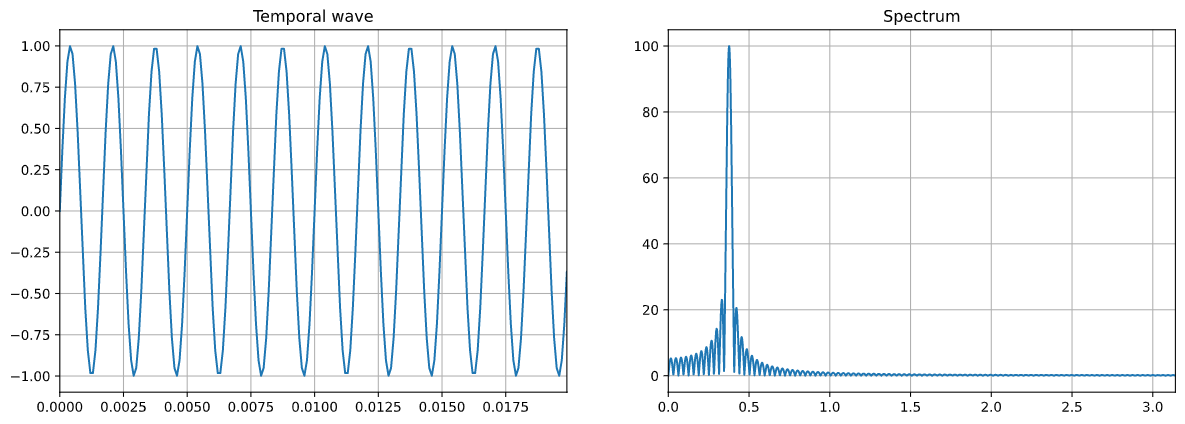
\includegraphics[scale=0.25]{q1.png}
\end{figure}

As expected, on the first graph, the maximum value is one and the minimun value is minus one corresponding to the amplitude=1 of the signal.
The sine wave also achieves 6 periods in 10 ms meaning that its frequency is $ 1000\frac{6}{10}=600 \text{Hz} $.
On the second graph, we observe a spike at $ \phi\approx0.376 $ which after computation gives us a frequency of $ f=600\text{Hz} $.

\section{Influence of the Sampling Frequency}
\subsection*{Question 2}


For $f=600Hz$ and $f=4400Hz$, we see that the Fourier transform corrrespond to the reality, because $2f \leq Fe$ (Shannon's theorem).  
For $f=5000Hz$, samples represents the sum of the errors. We should see a graph with 0 everywhere if errors were equals to 0, because $2f = Fe$.  
For $f=5600Hz$ and $f=10600Hz$, we observe a stroboscopic effect because $2f > Fe$. So the Fourier transform doesn't correspond to the reality.

\begin{figure}[H]
    \centering
    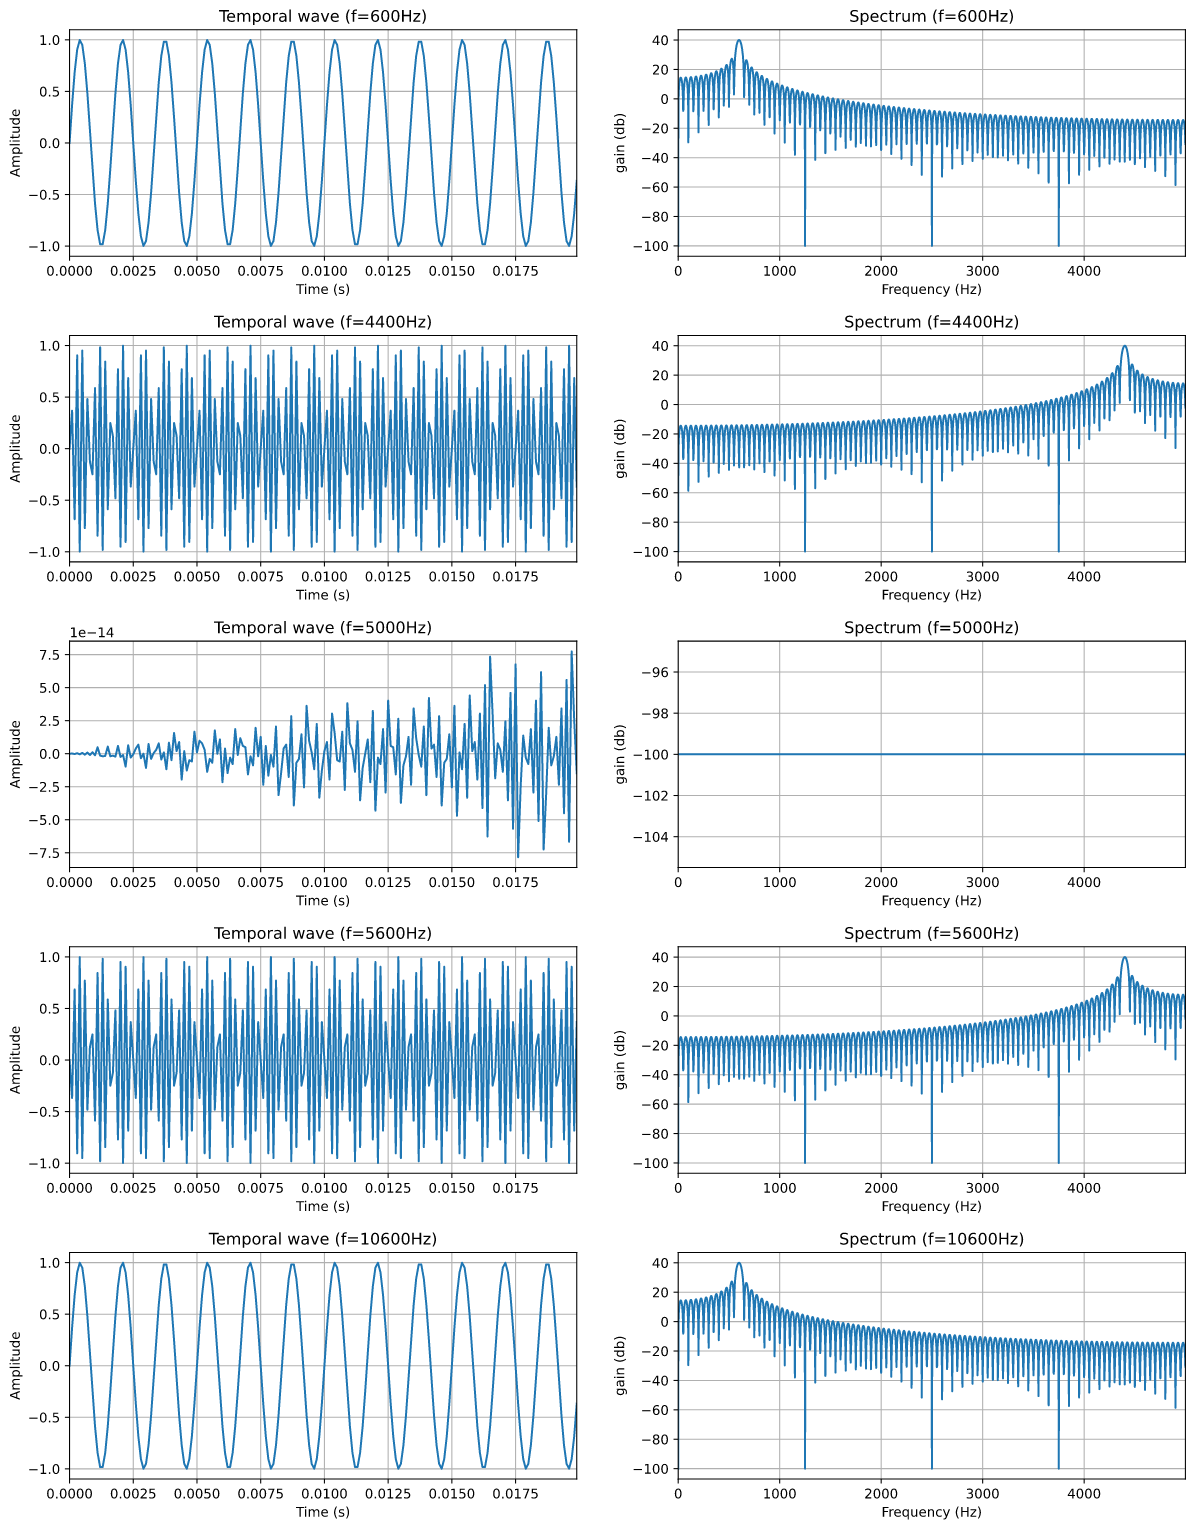
\includegraphics[scale=0.25]{q2.png}
\end{figure}

\section{Influence of the Parameter NTFD}
\subsection*{Question 3}


\begin{enumerate}
    \item \begin{enumerate}
        \item The Position of the Fourier spike is at $2\pi*\frac{f}{F_e} = 1.66$.
        \item The maximum of the Fourier spike is equal to $\frac{N}{2}=16$.
        \item There are two frequency samples on each secondary lobe.
    \end{enumerate}
    \item \begin{enumerate}
        \item The position of the Fourier spike is at $2\pi*\frac{f}{F_e} = 1.66$.
        \item The maximum of the Fourier spike is equal to $\frac{N}{2}=16$.
        \item There are sixteen frequency samples on each secondary lobe.
    \end{enumerate}
    \item \begin{enumerate}
        \item The position of the Fourier spike is at $2\pi*\frac{f}{F_e} = 1.57$.
        \item The maximum of the Fourier spike is equal to $\frac{N}{2}=16$.
        \item There are two frequency samples on each secondary lobe.
    \end{enumerate}
    \item \begin{enumerate}
        \item The position of the Fourier spike is at $2\pi*\frac{f}{F_e} = 1.57$.
        \item The maximum of the Fourier spike is equal to $\frac{N}{2}=16$.
        \item There are sixteen frequency samples on each secondary lobe.
    \end{enumerate}
\end{enumerate}

\begin{figure}[H]
    \centering
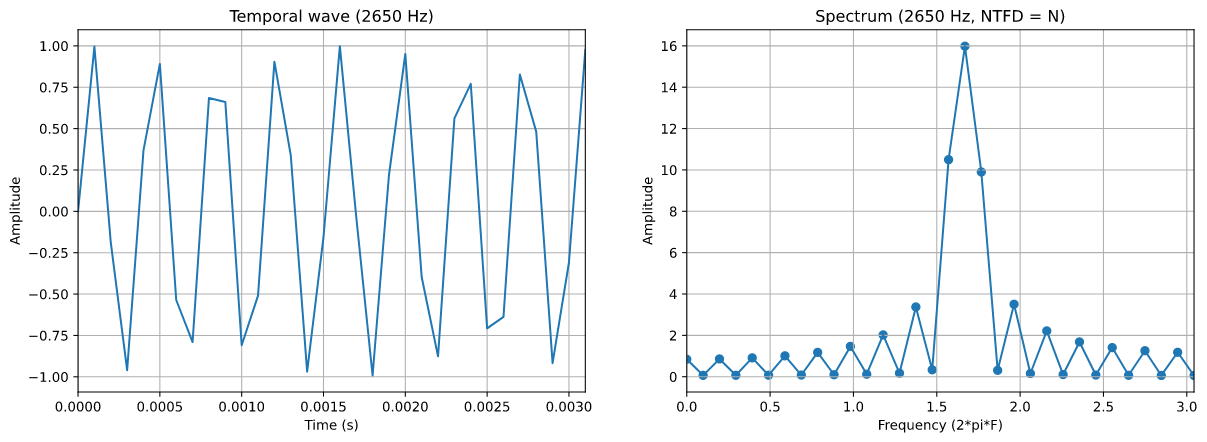
\includegraphics[scale=0.25]{q31.png}\\
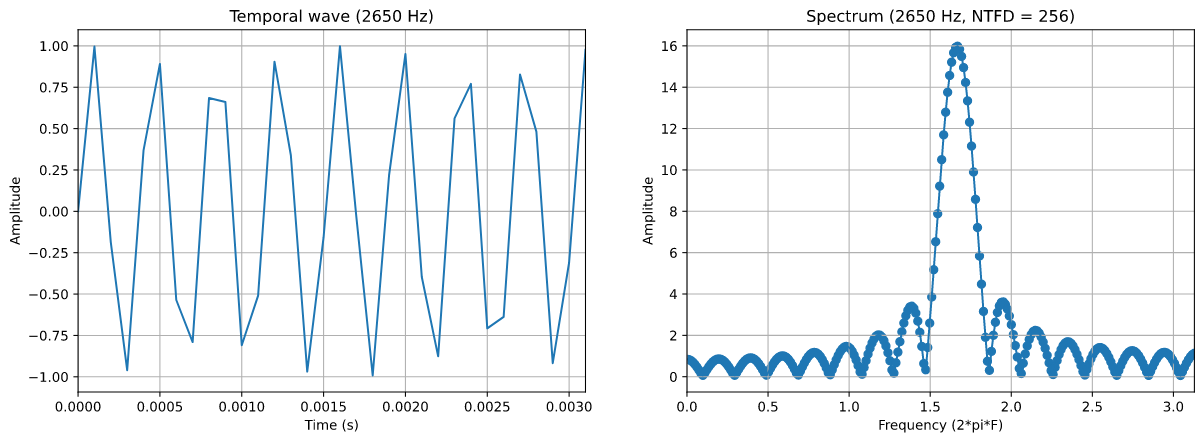
\includegraphics[scale=0.25]{q32.png}\\
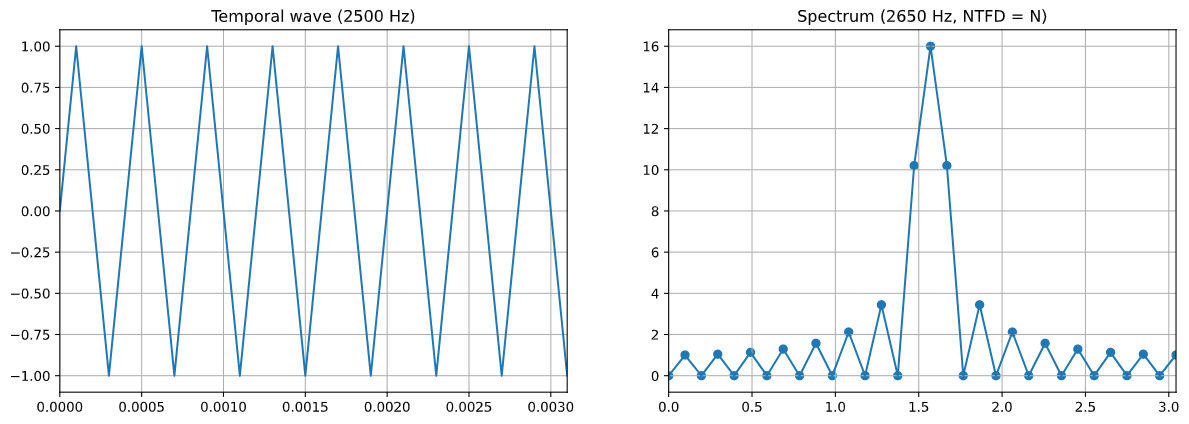
\includegraphics[scale=0.25]{q33.png}\\
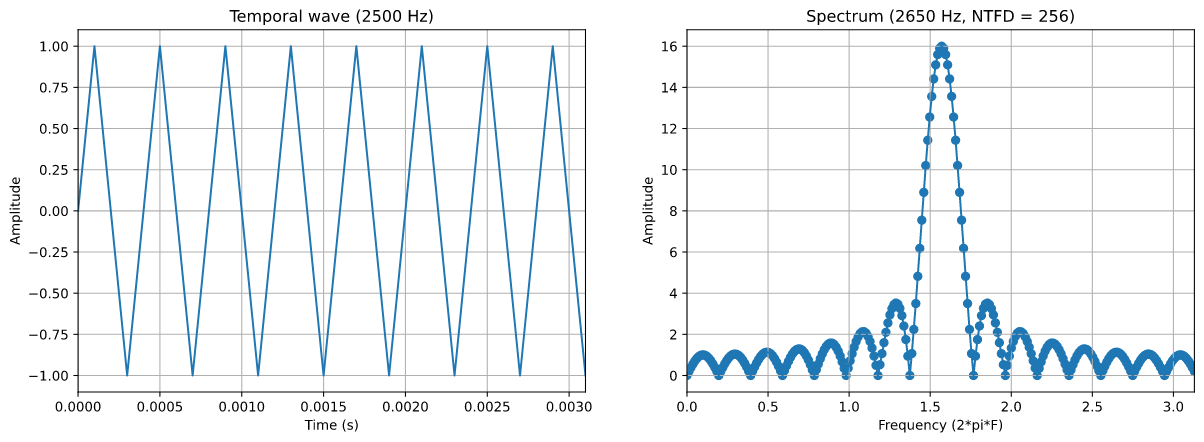
\includegraphics[scale=0.25]{q34.png}\\
\end{figure}

\section{Spectral Analysis of Several Sine Waves}
\subsection*{Question 4}

We find that the closer the sample frequency is to twice the higher frequency, the closer the spikes are to pi.
So in order to increase the accuracy, it's better to set the sample rate as close as possible
to two times the higher frequency that we want to observe. 
For the NTFD parameter, that only change the space between the frequency samples in the spectrum.
So, the higher it is the most continuous the plot seems. 
For the number of samples in the time's space, we observe that the shorter the signal lasts in time the larger the spike corresponding to
that signal frequency is and vice versa. There is probably a link with the uncertainty principle in quantum mechanics.


\section{Weighting Window Effect}
\subsection*{Question 5}

\begin{figure}[H]
    \centering
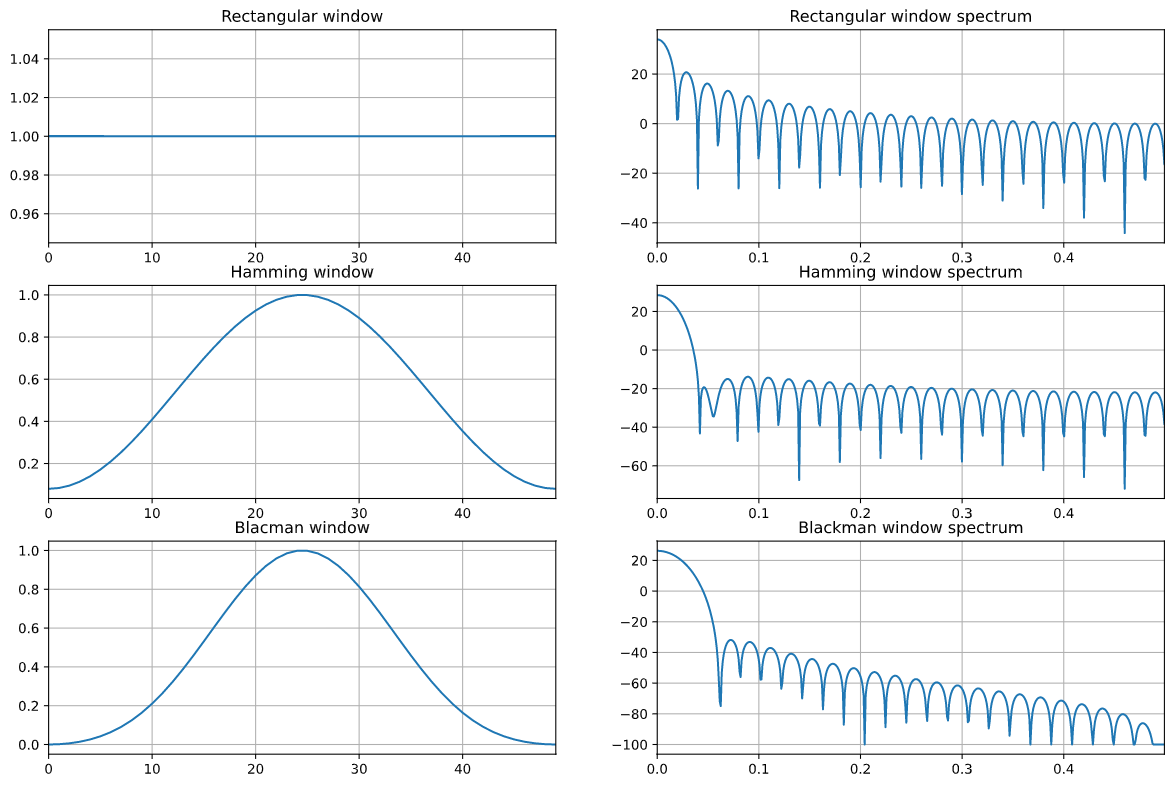
\includegraphics[scale=0.25]{q5.png}
\end{figure}

We observe that the main lobe is getting larger and larger and the other lobes are getting lower and lower from one window to another.
That fits well with the given table.

\subsection*{Question 6}


For the first signal, the rectangular window seems to be the least bad one. For the second sinusoid, it's the Blackman window which does the better job. But we don't know why.

\begin{figure}[H]
    \centering
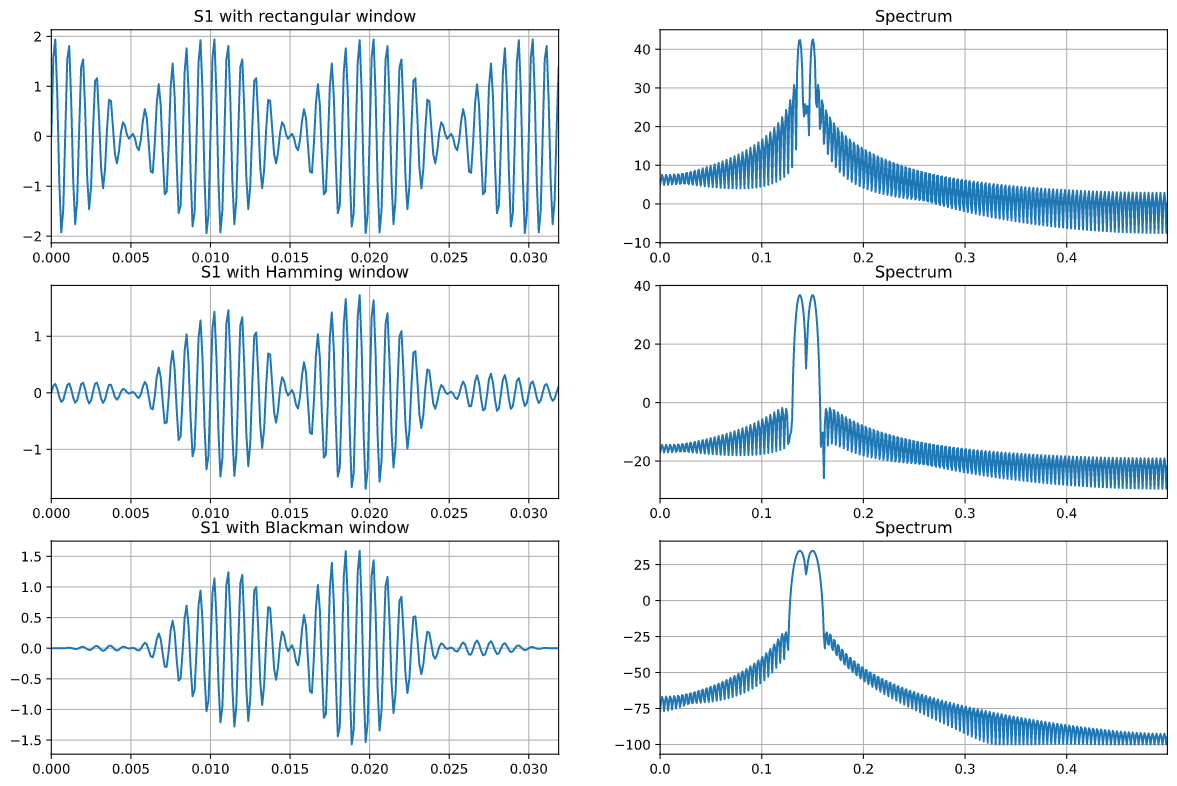
\includegraphics[scale=0.25]{q61.png}
\end{figure}

\begin{figure}[H]
    \centering
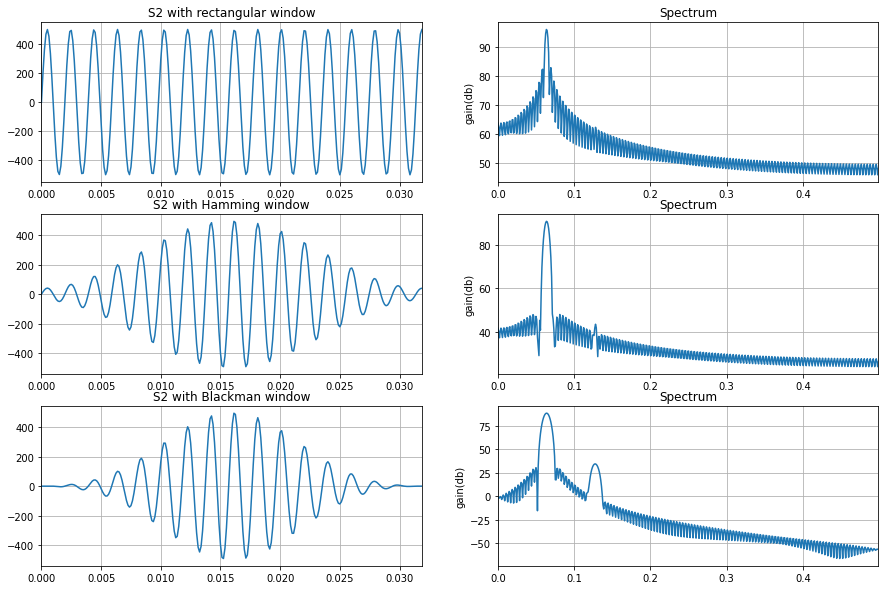
\includegraphics[scale=0.25]{q62.png}
\end{figure}

\end{document}